%% bare_conf.tex
%% V1.3


% Note that the a4paper option is mainly intended so that authors in
% countries using A4 can easily print to A4 and see how their papers will
% look in print - the typesetting of the document will not typically be
% affected with changes in paper size (but the bottom and side margins will).
% Use the testflow package mentioned above to verify correct handling of
% both paper sizes by the user's LaTeX system.
%
% Also note that the "draftcls" or "draftclsnofoot", not "draft", option
% should be used if it is desired that the figures are to be displayed in
% draft mode.
%
\documentclass[a4paper,conference]{IEEEtran}


% *** CITATION PACKAGES ***
%
\usepackage{cite}
% cite.sty was written by Donald Arseneau
% V1.6 and later of IEEEtran pre-defines the format of the cite.sty package
% \cite{} output to follow that of IEEE. Loading the cite package will
% result in citation numbers being automatically sorted and properly
% "compressed/ranged". e.g., [1], [9], [2], [7], [5], [6] without using
% cite.sty will become [1], [2], [5]--[7], [9] using cite.sty. cite.sty's
% \cite will automatically add leading space, if needed. Use cite.sty's
% noadjust option (cite.sty V3.8 and later) if you want to turn this off.
% cite.sty is already installed on most LaTeX systems. Be sure and use
% version 4.0 (2003-05-27) and later if using hyperref.sty. cite.sty does
% not currently provide for hyperlinked citations.
% The latest version can be obtained at:
% http://www.ctan.org/tex-archive/macros/latex/contrib/cite/
% The documentation is contained in the cite.sty file itself.






% *** GRAPHICS RELATED PACKAGES ***
%
\ifCLASSINFOpdf
   \usepackage[pdftex]{graphicx}
  % declare the path(s) where your graphic files are
   \graphicspath{{./}}
  % and their extensions so you won't have to specify these with
  % every instance of \includegraphics
  \DeclareGraphicsExtensions{.pdf,.jpeg,.png}
\else
  % or other class option (dvipsone, dvipdf, if not using dvips). graphicx
  % will default to the driver specified in the system graphics.cfg if no
  % driver is specified.
  % \usepackage[dvips]{graphicx}
  % declare the path(s) where your graphic files are
  % \graphicspath{{../eps/}}
  % and their extensions so you won't have to specify these with
  % every instance of \includegraphics
  % \DeclareGraphicsExtensions{.eps}
\fi




\usepackage[cmex10]{amsmath}



\usepackage{algorithmic}




% *** ALIGNMENT PACKAGES ***
%
\usepackage{array}


\usepackage{mdwmath}
\usepackage{mdwtab}




% *** SUBFIGURE PACKAGES ***
\usepackage[tight,footnotesize]{subfigure}
% subfigure.sty was written by Steven Douglas Cochran. This package makes it
% easy to put subfigures in your figures. e.g., "Figure 1a and 1b". For IEEE
% work, it is a good idea to load it with the tight package option to reduce
% the amount of white space around the subfigures. subfigure.sty is already
% installed on most LaTeX systems. The latest version and documentation can
% be obtained at:
% http://www.ctan.org/tex-archive/obsolete/macros/latex/contrib/subfigure/
% subfigure.sty has been superceeded by subfig.sty.



\usepackage[caption=false]{caption}
\usepackage[font=footnotesize]{subfig}
% subfig.sty, also written by Steven Douglas Cochran, is the modern
% replacement for subfigure.sty. However, subfig.sty requires and
% automatically loads Axel Sommerfeldt's caption.sty which will override
% IEEEtran.cls handling of captions and this will result in nonIEEE style
% figure/table captions. To prevent this problem, be sure and preload
% caption.sty with its "caption=false" package option. This is will preserve
% IEEEtran.cls handing of captions. Version 1.3 (2005/06/28) and later 
% (recommended due to many improvements over 1.2) of subfig.sty supports
% the caption=false option directly:
%\usepackage[caption=false,font=footnotesize]{subfig}
%
% The latest version and documentation can be obtained at:
% http://www.ctan.org/tex-archive/macros/latex/contrib/subfig/
% The latest version and documentation of caption.sty can be obtained at:
% http://www.ctan.org/tex-archive/macros/latex/contrib/caption/




% *** FLOAT PACKAGES ***
%
\usepackage{fixltx2e}
% fixltx2e, the successor to the earlier fix2col.sty, was written by
% Frank Mittelbach and David Carlisle. This package corrects a few problems
% in the LaTeX2e kernel, the most notable of which is that in current
% LaTeX2e releases, the ordering of single and double column floats is not
% guaranteed to be preserved. Thus, an unpatched LaTeX2e can allow a
% single column figure to be placed prior to an earlier double column
% figure. The latest version and documentation can be found at:
% http://www.ctan.org/tex-archive/macros/latex/base/



%\usepackage{stfloats}
% stfloats.sty was written by Sigitas Tolusis. This package gives LaTeX2e
% the ability to do double column floats at the bottom of the page as well
% as the top. (e.g., "\begin{figure*}[!b]" is not normally possible in
% LaTeX2e). It also provides a command:
%\fnbelowfloat
% to enable the placement of footnotes below bottom floats (the standard
% LaTeX2e kernel puts them above bottom floats). This is an invasive package
% which rewrites many portions of the LaTeX2e float routines. It may not work
% with other packages that modify the LaTeX2e float routines. The latest
% version and documentation can be obtained at:
% http://www.ctan.org/tex-archive/macros/latex/contrib/sttools/
% Documentation is contained in the stfloats.sty comments as well as in the
% presfull.pdf file. Do not use the stfloats baselinefloat ability as IEEE
% does not allow \baselineskip to stretch. Authors submitting work to the
% IEEE should note that IEEE rarely uses double column equations and
% that authors should try to avoid such use. Do not be tempted to use the
% cuted.sty or midfloat.sty packages (also by Sigitas Tolusis) as IEEE does
% not format its papers in such ways.





% *** PDF, URL AND HYPERLINK PACKAGES ***
%
%\usepackage{url}
% url.sty was written by Donald Arseneau. It provides better support for
% handling and breaking URLs. url.sty is already installed on most LaTeX
% systems. The latest version can be obtained at:
% http://www.ctan.org/tex-archive/macros/latex/contrib/misc/
% Read the url.sty source comments for usage information. Basically,
% \url{my_url_here}.



% *** Do not adjust lengths that control margins, column widths, etc. ***
% *** Do not use packages that alter fonts (such as pslatex).         ***
% There should be no need to do such things with IEEEtran.cls V1.6 and later.
% (Unless specifically asked to do so by the journal or conference you plan
% to submit to, of course. )


% correct bad hyphenation here
\hyphenation{op-tical net-works semi-conduc-tor}


\begin{document}
%
% paper title
% can use linebreaks \\ within to get better formatting as desired
\title{Random Access Mechanisms for \\ DNA Storage Systems}


% author names and affiliations
% use a multiple column layout for up to three different
% affiliations
\author{\IEEEauthorblockN{Ryan Quinn Ford}
\IEEEauthorblockA{Philipps-University Marburg, Germany \\
Department of Mathematics and Computer Science, Distributed Systems Group \\
Email: ford@informatik.uni-marburg.de
}}

% conference papers do not typically use \thanks and this command
% is locked out in conference mode. If really needed, such as for
% the acknowledgment of grants, issue a \IEEEoverridecommandlockouts
% after \documentclass

% for over three affiliations, or if they all won't fit within the width
% of the page, use this alternative format:
% 
%\author{\IEEEauthorblockN{Michael Shell\IEEEauthorrefmark{1},
%Homer Simpson\IEEEauthorrefmark{2},
%James Kirk\IEEEauthorrefmark{3}, 
%Montgomery Scott\IEEEauthorrefmark{3} and
%Eldon Tyrell\IEEEauthorrefmark{4}}
%\IEEEauthorblockA{\IEEEauthorrefmark{1}School of Electrical and Computer Engineering\\
%Georgia Institute of Technology,
%Atlanta, Georgia 30332--0250\\ Email: see http://www.michaelshell.org/contact.html}
%\IEEEauthorblockA{\IEEEauthorrefmark{2}Twentieth Century Fox, Springfield, USA\\
%Email: homer@thesimpsons.com}
%\IEEEauthorblockA{\IEEEauthorrefmark{3}Starfleet Academy, San Francisco, California 96678-2391\\
%Telephone: (800) 555--1212, Fax: (888) 555--1212}
%\IEEEauthorblockA{\IEEEauthorrefmark{4}Tyrell Inc., 123 Replicant Street, Los Angeles, California 90210--4321}}




% use for special paper notices
%\IEEEspecialpapernotice{(Invited Paper)}




% make the title area
\maketitle


\begin{abstract}
%\boldmath
With the global amount of data growing at a speed which current storage technologies cannot hold pace with, researchers have looked to DNA for a novel storage solution. DNA provides an unprecedented data density and long-term durability, which is now being actualized for data storage thanks to ever-decreasing sequencing costs. Due to very low read speeds and delicate conditions, it is of significant importance to find ways to more efficiently randomly access data in a DNA store, e.g. retrieving values from keys. In this paper I discuss three recent breakthroughs in techniques for random access in DNA storage and their capabilities and outlook in regards to scalability and error correction/detection. In addition, I will take a look at the current limitations that face these techniques and what areas they open up to future research.
\end{abstract}
% IEEEtran.cls defaults to using nonbold math in the Abstract.
% This preserves the distinction between vectors and scalars. However,
% if the conference you are submitting to favors bold math in the abstract,
% then you can use LaTeX's standard command \boldmath at the very start
% of the abstract to achieve this. Many IEEE journals/conferences frown on
% math in the abstract anyway.

% no keywords




% For peer review papers, you can put extra information on the cover
% page as needed:
% \ifCLASSOPTIONpeerreview
% \begin{center} \bfseries EDICS Category: 3-BBND \end{center}
% \fi
%
% For peerreview papers, this IEEEtran command inserts a page break and
% creates the second title. It will be ignored for other modes.
\IEEEpeerreviewmaketitle



\section{Introduction}
% no \IEEEPARstart
% You must have at least 2 lines in the paragraph with the drop letter
% (should never be an issue)
As this paper is intended for an audience with a computer science background, it is necessary to touch upon some underlying biological principles. Additionally, a brief overview of relevant database system concepts will be given. The following sections of the introduction do these, which gives us the terminology we need to achieve a deeper understanding of the biochemical and information theoretical constraints that apply.

\subsection{High-Level Overview and Reasoning}
Many properties of DNA have led it to be considered as an innovative candidate for data storage, which has led it to become a heavily researched topic over the past decade. The amount of stored data in the world is growing at a rate of 30\% to 40\% a year \cite{globaldatagrowth}, outpacing the growth of today's current storage medium's capabilities. As a result, researchers have recently looked towards new mediums to remedy this problem. DNA sequencing and accompanying technologies have experienced significant cost reduction in past years, making DNA an increasingly attractive medium for the future. 

To understand the appeal, one can first contemplate the theoretical bounds for storage data in a DNA molecule.  An estimate of the information capacity considering reasonable encoding constraints is 1.83 bits per nucleotide \cite{1}, which may sound uninteresting as a storage medium until the physical size of this structure is considered.  A single base pair has a mass of about 330g/mol \cite{2}, which results in a storage capacity of 137.76 zettabytes per gram. This is an improvement of many orders of magnitude over current long term storage mediums, such as magnetic tape \cite{?}.\\

Another appealing aspect of DNA storage is it's robustness. With a half life of 521 years \cite{dnahalflife}, a DNA strand will persist for around 6.8 million years. The current best option for long term data storage is magnetic tape, which, must be replaced around every 10 years.

Random access of data storage is a crucial property regarding the usability of any storage system, even for archival storage. Without random access, one would have to read and decode an entire DNA database before being able to read a single file or data segment. In computer systems one can use physical addresses of data segments for later access, but in a DNA storage the physical location of the searched strand is unknown. 

Once data was first successfully stored into DNA and successfully retrieved, the focus became directed at the scalability of these storage systems. Random access of the system goes hand in hand with its scalability, as the more data is stored, the more difficult it becomes to retrieve.

%{dnahalflife}https://royalsocietypublishing.org/doi/10.1098/rspb.2004.3016

%\hfill mds
 
%\hfill January 11, 2007

\subsection{Underlying Biological Concepts}

\begin{center}
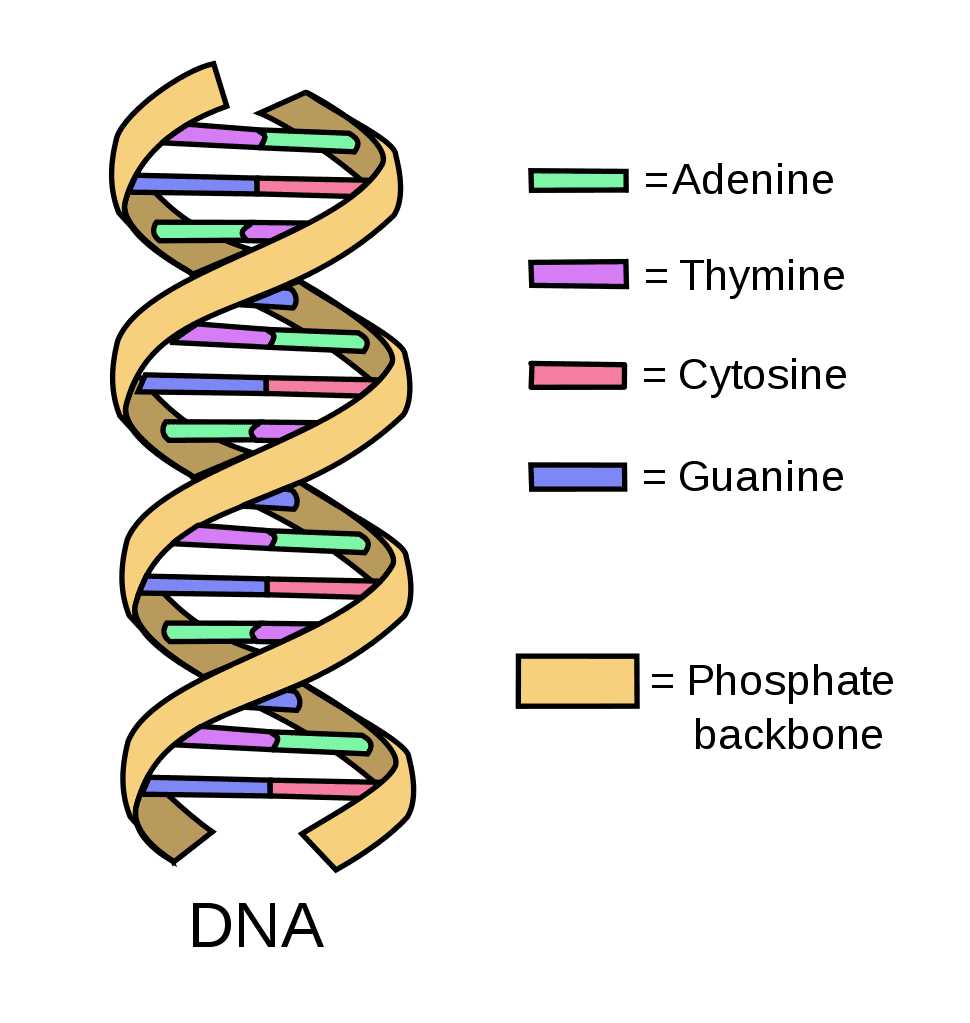
\includegraphics[width=2in]{dna}
\end{center}


\subsubsection{DNA Basics}
Deoxyribonucleic Acid, more commonly referred to as \textbf{DNA}, is the carrier of genetic information in all living beings and our storage medium of interest. A strand of DNA is comprised of four chemical building blocks called \textbf{nucleotides} which occur sequentially in a strand, connected by a sugar-phosphate backbone. Such a strand of nucleotides is commonly referred to as an \textbf{oligo}, short for oligonucleotide.

Each DNA strand has two chemically distinct ends, called 5' and 3', and is made up of nucleotides, also called \textbf{bases}, which are named Adenine, Thymine, Guanine, and Cytosine, and are abbreviated as A, T, G, and C, respectively. Each pairing in a DNA molecule is called a \textbf{base pair} (bp). In these canonical base pairings, Adenine pairs with Thymine, and Guanine pairs with Cytosine. A strand's reverse complement is defined as its sequence of complementary base pairs and swapped 3' and 5' ends.

The primary structure of a DNA molecule is a double-helix, discovered by Watson and Crick in \cite{3}. In this structure, two reversely complementary strands bind to each other in a "twisted ladder" formation, where each nucleotide on one side forms a hydrogen bond with the one on the opposing side in one of two of the canonical pairings. Two bound, complementary strands can be referred to as ds-DNA (doubly stranded DNA), while a single strand can be referred to as ss-DNA (singly stranded DNA).

\subsubsection{RNA}

DNA stores all biological information of an organism, including the instructions for the creation of proteins. A specific protein called an RNA polymerase creates a different chain of nucleotides referred to as RNA. In contrast to the DNA polymerase, the RNA polymerase needs a DNA strand to assemble the corresponding RNA sequence. Although RNA serves many functions, for our purposes, it is only relevant to regard a few aspects which sets RNA apart from DNA.

\begin{itemize}
    \item Thymine is replaced with Uracil as the base pairing for Adenine. This means RNA consists of the bases A, U, G, and C.
    \item RNA is single stranded, but still often folds on itself to minimize it's free energy. This creates secondary structures, which will be discussed in more detail later.
    \item The RNA polymerase generates RNA from a DNA strand without breaking apart the double helix structure at the same time. The molecule goes down a region of DNA like a zipper, both opening up the DNA and closing it as it travels across.
\end{itemize}

\subsection{Biochemical Limitations Leading to Errors}
DNA is a living molecule, so it is unwise to map data to it without first taking some biochemical limitations into consideration.

\subsubsection{Homopolymers}
One of such limitations stems from \textbf{homopolymers}, regions of a strand which solely consist of repetitions of a single base. It is of critical importance to avoid such homopolymers in the encoding process, as they render a strand more error prone \cite{?} and unstable.

\subsubsection{GC Content}
Another important property of a DNA strand is its \textbf{GC Content}, which is defined as the ratio of Guanine and Cytosine bases to the total count of bases in the strand. Having a reasonable GC Content \cite{?} is important to the strand's stability. 


\subsubsection{Secondary Structures}
Yet another limitation to be considered is the formation of secondary structures. Secondary structures form when a DNA strand binds to itself or another semi-complementary strand in an undesirable way. For example, if a ss-DNA strand contains a region of its own reverse complement, the strand can bind to itself instead of to a separate complementary strand. This causes an issue for the DNA polymerase molecule in PCR, which will be discussed later, because it is not able to unbind the strand from itself.

\subsection{DNA in storage}
A container of solution containing ds-DNA molecules is called a DNA pool. Most often, the entirety of the data is not stored in a single container, but rather divided up into many DNA pools in order to avoid the aforementioned conflicts, especially undesirable binding to incorrect data fragments.

\subsection{Random Access}
\begin{figure}
\centering
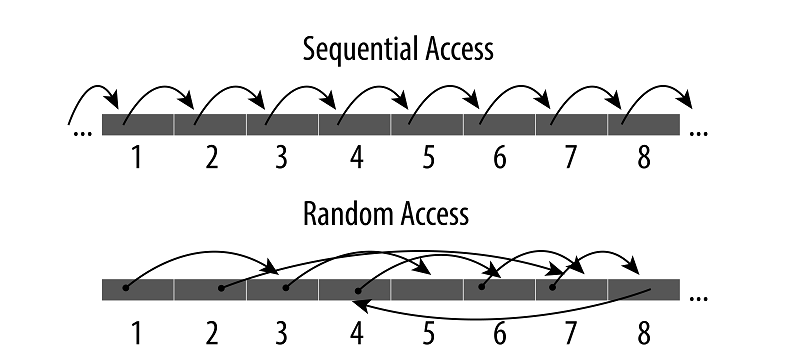
\includegraphics[width=3.5in]{randomaccess}
\caption{Random Access}
\label{randomaccess}
\end{figure}

Random (direct) access in a storage system implies the ability to access all data fragments in any arbitrary order. In order to randomly access data from a DNA library, multiple properties must exist on the encoded strands:

\subsubsection{Uniquely Addressable}
There must be a distinct property of each stored information strand that allows it to be identified independently from all other strands. This means for any given information-bearing strand, there must be a process that sets it apart from all other strands, allowing it to be targeted.
\subsubsection{Targetable}
For random access one must also be capable of targeting the individual addresses of all sequences. This simply means that given a DNA pool, there must be a mechanism that "searches" for a given strand independently from it's neighbors.
\subsubsection{Readable}
Once the searched strand is targeted, it must be read by some process. In the context of DNA pools, this property is given by the used sequencing technology.



%[1] https://www.biorxiv.org/content/10.1101/074237v3.full.pdf
%[2] https://www.sciencedirect.com/science/article/abs/pii/S0022283662801004?via%3Dihub

%\subsubsection{Deoxyribonucleic Acid}
%Subsubsection text here.


\subsection{Encoding Data into DNA}
In order to store data into a DNA strand, one must first consider how the data gets mapped to the four available bases. This process will be referred to as encoding. On first glance, one may try assigning each of the four bases a two bit sequence, for example A=00, C=01, T=10, G=11. This simple mapping would mean a byte like 01100011 would get transformed into the base sequence CTAG. Depending on the data format, regions of the binary representation may often repeat itself heavily. If one were to map two bits per base naively as described, this would result in highly error prone strands due to extreme GC Content and long homopolymer regions, among other issues. For these reasons, two main operations are performed on the data in the majority of previous work.

\subsubsection{XOR}
When encoding a library of data, it must be broken up into smaller chunks. This is because costs increase prohibitively with each added base, and with each added base comes more chances for errors to occur which can propagate upwards and cause catastrophic failure at sequencing. Because digital data is non-random, i.e., much of the data we want to store is repetitive and redundant, many of the chunked sequences would get encoded similar to each other. If this were done without care, the sequences would not bind to their respective complementary strand but rather incompletely to similar strands. This is what is meant with maximizing the orthogonality of the strands.

For this reason, a extra precaution is often taken as a first step, in which the bit sequence is XOR'ed with a psuedo-randomly generated sequence which can later be recovered. This ensures that two similar sequences get encoded in different ways. One can consider this as a very simple hashing mechanism. Of course, this psuedo-random sequence must later be regenerated in order to reverse this process (which happens with a second XOR operation in exactly the same way).

\subsubsection{Rotating Huffman Code}
One of the most obvious improvements to make would be to take lessons learned from information theory into account and make sure that the encoding doesn't take up more bits than necessary. Not only does this reduce costs, but also reduces the probability of errors. As stated above, much of digital data is repetitive and redundant. For this, lossless compression using Huffman coding as seen in \ref{code} has been used in the vast majority of recent works.

In Huffman coding, a byte sequence is separated into $n$-ary sequences and the relative frequencies of each sequence is calculated. In our case, we use triplets of bits. A binary tree is then generated assigning more probable triplets codes of shorter length in order to store the data more efficiently.

This process alone, however, does not remedy the problem of repetitive regions. For this, a rotating code is used, which simply ensures that the same base is never repeated more than once. This is achieved by not only choosing the base based on the ternary digit from the Huffman code, but also based on the previous nucleotide.

Combining these two methods allows for a sequence which fares relatively well in reducing homopolymer count and keeping GC content at around 50\%.




\begin{figure}
\centering
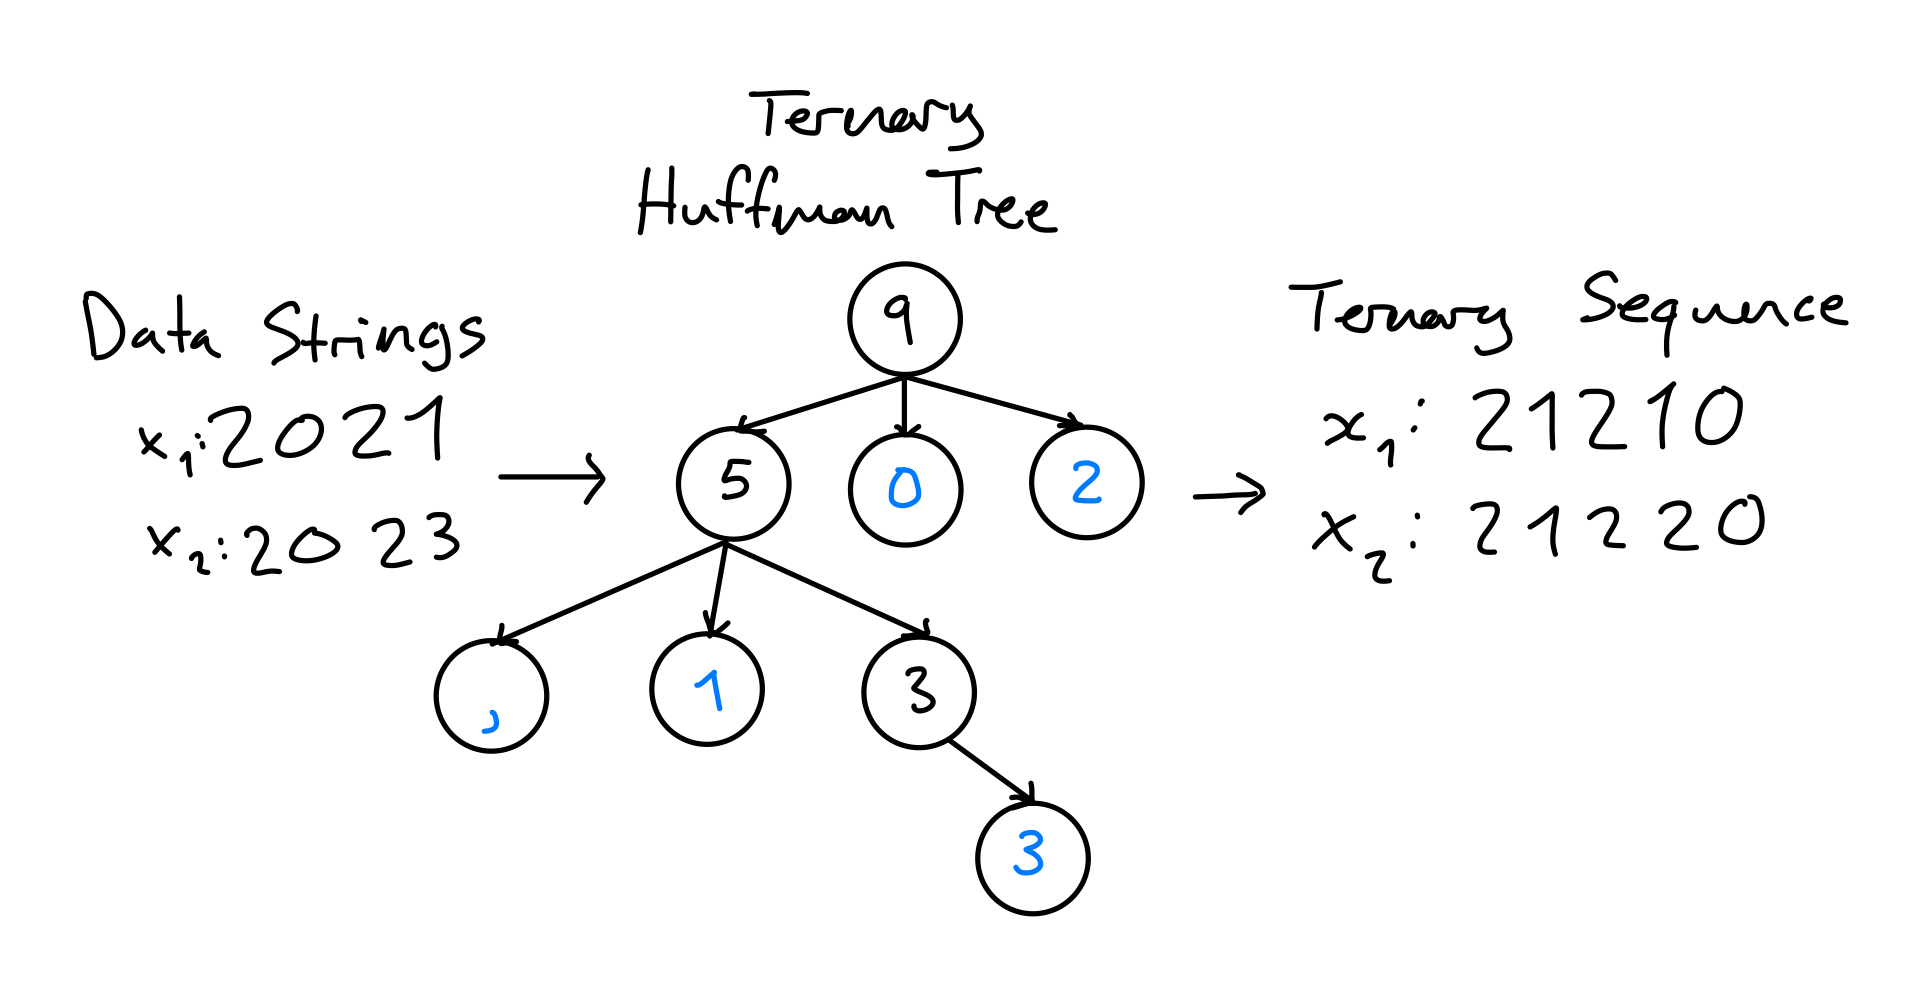
\includegraphics[width=3.5in]{huffman}
\caption{Ternary Huffman Code}
\label{code}
\end{figure}
\begin{figure}
\centering
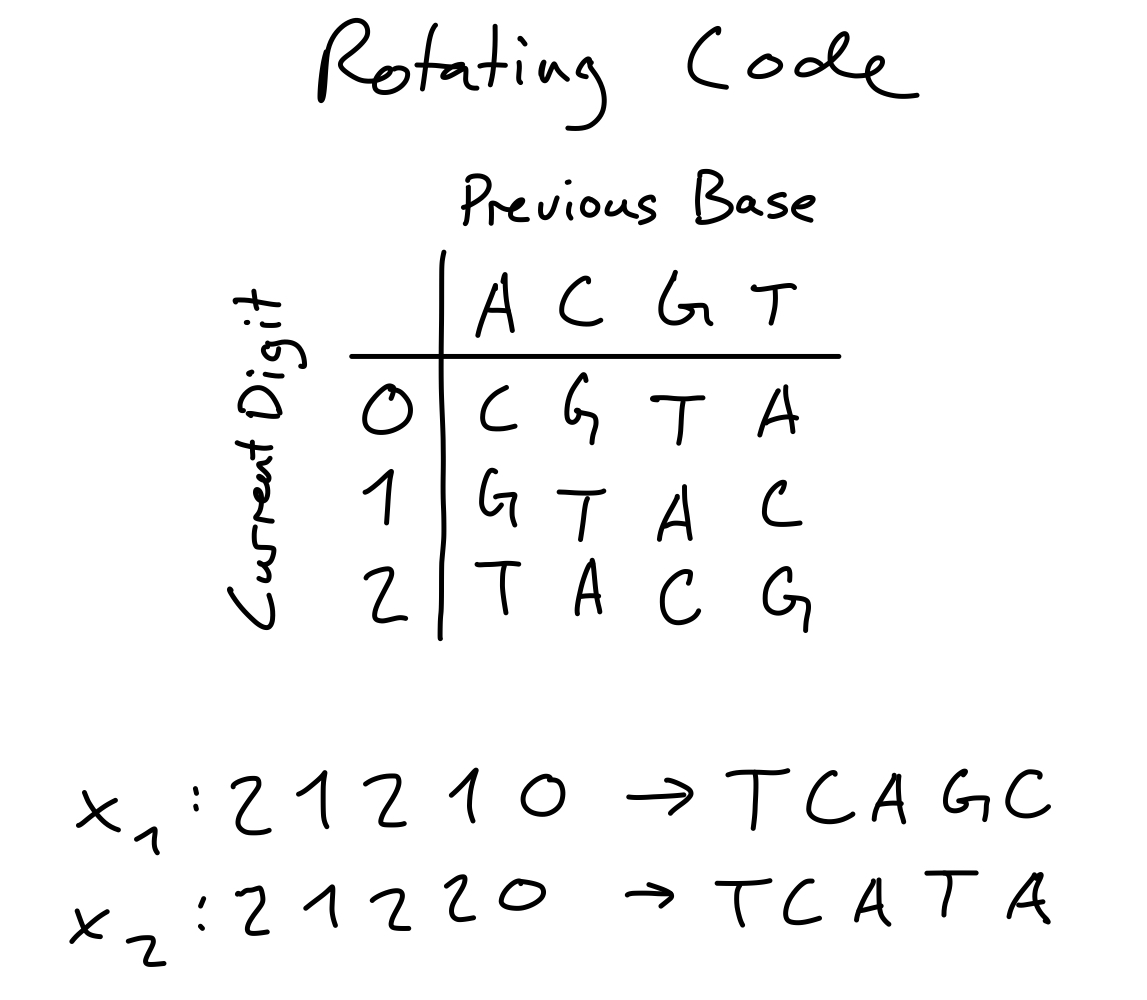
\includegraphics[width=2.5in]{rotatingcode}
\caption{Rotating Code}
\label{code}
\end{figure}

\subsubsection{Erasure Codes}
Due to high error rates when reading the DNA, there must be some redundancy to ensure the data is properly recovered. This is commonly implemented with erasure codes, in which the data sequence is transformed into a longer sequence which can be successfully decoded with only a subset of the characters from the encoding. In current DNA libraries, the redundancy parameter is tuned relatively high \cite{}, which significantly reduces the achieved information density. As sequencing technology improves, the redundancy parameter should be able to be tuned down \cite{} due to lower read errors and improved encoding schemes which are aware of and avoid secondary structure formation.

In the works we will discuss the most common erasure code used is the Reed-Solomon code. The Reed-Solomon Code is a type of erasure code that comprise of an inner and outer redundancy component. This technique has been widely adopted in digital systems and results in massive gains in regards to the recoverability of data as well as the correction of errors in it.



\begin{figure}[!t]
\centering
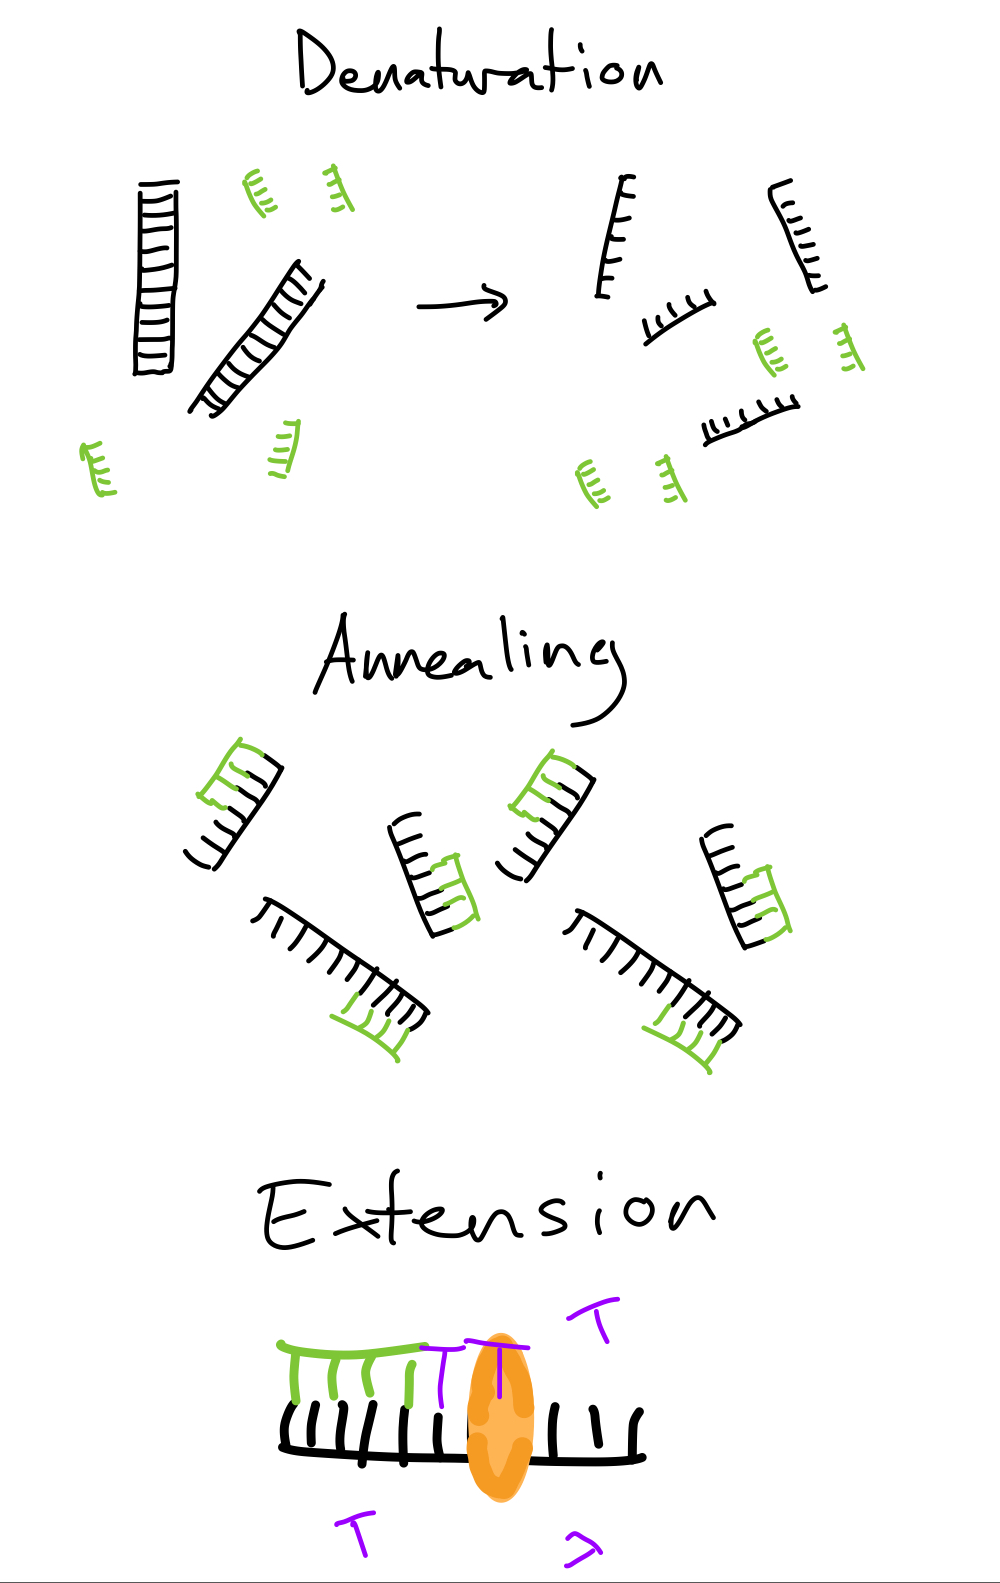
\includegraphics[width=3.5in]{pcr}
\caption{PCR Stages}
\label{fig_sim}
\end{figure}

\subsection{Introduction to PCR}

After the data has been mapped to a DNA strand, it is time to synthesize the sequences and prepare them for storage. One aspect of this preparation often involves PCR (Polymerase Chain Reaction), in which each DNA sequence is multiplied millions of times. PCR is necessary both to create physical redundancy and as we will discuss later, as a random access mechanism. In this process, after the data has been mapped to the four nucleotides as discussed above, a so-called primer is appended to the sequence. This primer will serve as a marker of the region to be copied by an enzyme called a DNA Polymerase. This copying, also called amplification, occurs in cycles involving the following steps. \\

\subsubsection{Denaturation}
In a process called denaturation, DNA molecules are split up into its two complementary strands by being heated to a target temperature $T_m$, called the \textit{melting point}. This melting point is defined as the temperature where 50\% of the DNA strands separate. This occurs because the heat breaks the hydrogen bonds holding the two strands together. This step is necessary in order to later allow the complementary primer sequences to attach to each strand. \\
\subsubsection{Annealing}
Once the DNA molecules are split, the environment is cooled back down in a process called annealing. Since the strands are not bound to anything anymore, there is room for the primer sequences to bond to the complementary primer regions we appended to our data-holding DNA strand.\\
\subsubsection{Extension}
The DNA polymerase enzyme now finds the primers added in the last step, and fills up the other half double-helix by adding free nucleotides from the solution one by one.\\
\subsubsection{Repetition}
Now that the polymerase has recreated the original double-helix, the process can cycle, restarting at the denaturation step. The number of copies doubles with each step, allowing for rapid growth.\\

\section{Current Random Access Techniques}
In the next section we will explore the three recent breakthroughs in random accessibility for DNA storage. Because the field is new, it is an open research question as to how random access can be improved upon from the encoding level in order to be scalable. The main bottleneck regarding the scalability of random access to date has been the random access mechanism, which poses a much larger optimization problem currently than that of the encoding schemes. In particular, improving upon storage architectures reduces the need for high redundancy and overly robust encoding procedures, as these mainly serve to reduce the problems that the mechanism itself poses. The current available random access mechanisms heavily rely on good primer/address design, orthogonality of the encoded sequences, physical separation of the data, and the amount of data in each storage unit.

\begin{figure}[!t]
\centering
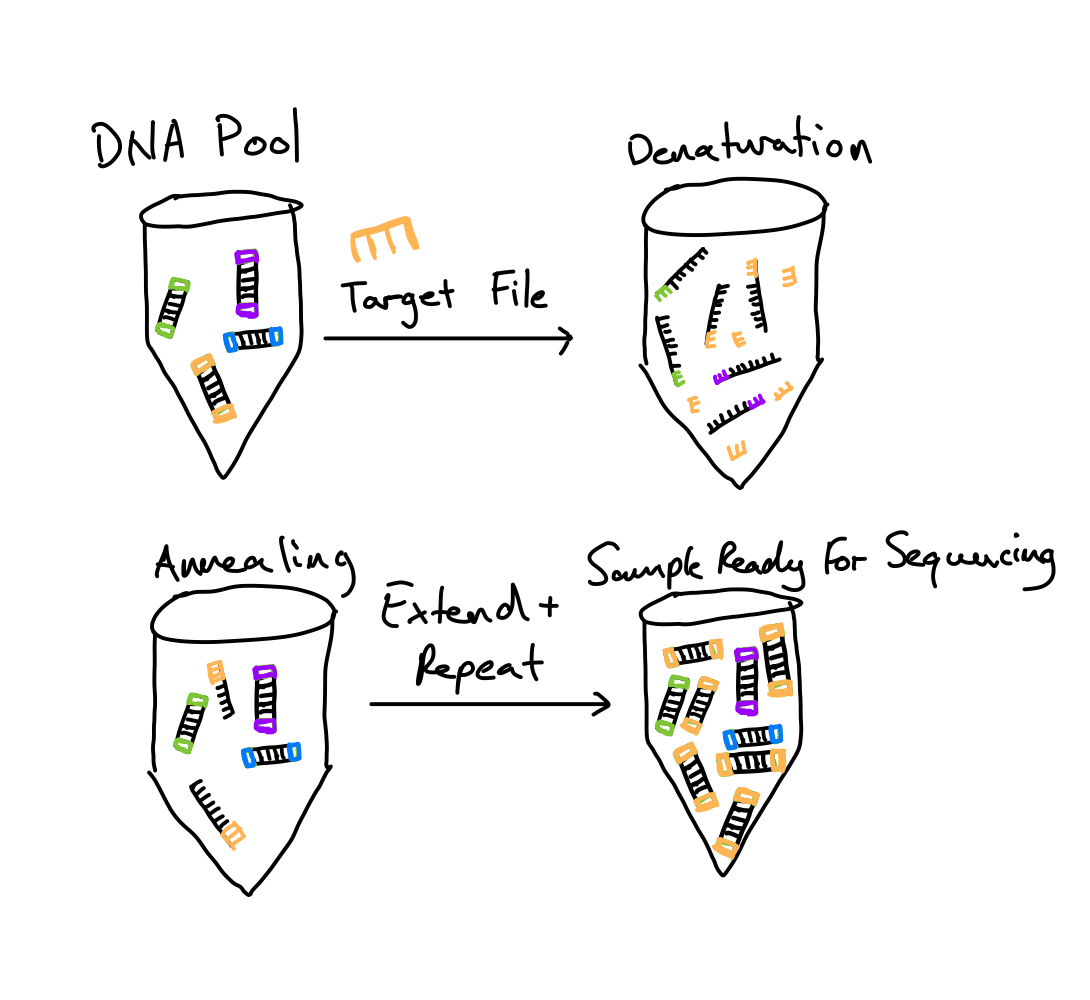
\includegraphics[width=3.5in]{pcrRA}
\caption{PCR in Random Access}
\label{fig_sim}
\end{figure}



\subsection{PCR Based Random Access}
The most basic form of random access in a DNA library comes from the separation of files into fragments, which all receive a distinct primer it can be identified by. Because this primer is stored in-silico, one can re-amplify the solution containing a specific DNA fragment on retrieval, effectively directly accessing the desired data. Nonetheless, primer design is a delicate task and the amount of primers that can be used is severely limited. This is partially alleviated by the breaking up of a dataset into $n$ physically separated DNA pools, allowing reuse of the primers and linearly scaling direct access capability to a certain threshold.

In this process, which I will refer to as PCR-Based random access, the PCR primers used for amplification before storage are utilized as the random access mechanism. This technique can be considered as the first generation, state-of-the art medium for random access in DNA storage. In previous works \cite{} this random access was achieved by separating the database into $n$ DNA pools, each with a given amount $k$ of amplified DNA fragments. Each of the $k$ fragments has a unique primer that was used for PCR amplification, so this is what is used as the address to later amplify and retrieve the correct fragment. The "targetable" property is achieved by the amplification of the strand to be read, effectively increasing the sequencing signal in comparison to the combination of the signals from all other neighboring strands. This is because sequencing technology is indifferent to which strands we have targeted and amplified, as it will read all stands in a sample anyways. However, because the desired strand has been amplified using its primer as an address, it can be distinguished from the other sequences.

Note that the scalability of this approach depends on the number of available primers, as these can only be reused once per pool for truly individually addressable files. This is the case for multiple reasons. For one, as discussed above, each random access requires sequencing of the entire DNA pool, since the targeted strands are not physically separated from the others. Any unamplified strands in the sample are destroyed upon sequencing, which dwindles the supply over time. In addition, the amount of information stored in a pool does not scale with the amount of primers, even in cases of exceptional primer design techniques. This is because the more sequences one adds to a pool, the more PCR cycles are needed to increase the signal of the queried strand high enough to complete a correct read. Finally, since PCR cycles involve repetitions of denaturation and annealing, any similarities between stored sequences will propagate errors due to unwanted interference through incorrect bindings and formations of secondary structures.

In \cite{}, Organick et. al. encoded and stored over 200MB of data spanning across 35 distinct files, each of which were recovered individually and without errors using PCR based random access. The main innovation presented in their work was showing the scalability of the PCR-based random access technique as well as the creation of a new algorithm to reduce the read coverage needed at sequencing. The new algorithm made it more practical to access a file from a pool by reducing the number of needed PCR cycles to amplify the queried data. This was also needed because sequencing is still heavily error prone \cite{}. Notably, their team was the first to prove that random access could be scaled up to a library size of 200MB and theoretically much higher.

Their DNA library consisted of more than 13 million DNA oligos in total. They encoded each digital file into megabyte sized blocks before encoding, appending the file address (PCR primer) to each block, then applying a Reed-Solomon Code. Before the data blocks were converted to nucleotides, an outer code was applied that added new blocks to the file containing redundant information. After this, an inner code is generated and applied to each bit sequence, in the process of which the bit string is translated into bases with added redundancy. 

To reduce the amount of needed cycles before sequencing, they also introduced an algorithm based on bitwise majority alignment (BMA), allowing one to more efficiently cluster the data from the noisy sequencing reads. This consists of four stages which will not be discussed here. The team tested their algorithm with both Illumna sequencing and micropore sequencing technologies, although Illumna sequencing was the main method used for the dataset.

In \cite{}, Yazdi et al. implement a comparable system, except with a focus on maximizing block length to reduce read errors instead of using shorter sequence lengths with higher redundancy. Because they had longer information strings in each sequence (1000bps), they were able to reach a higher information density of $4.9 \times 10^{20}$ B/g. They argue, "Instead of storing blocks mimicking the structure and length of reads generated during high-throughput sequencing, we synthesized blocks of length 1000bps tagged at both ends by specially designed address sequences. Adding addresses to short blocks of length 100bps would incur a large storage overhead, while synthesizing blocks longer than 1000bps using current technologies is prohibitively costly." In contrast to \cite{}, \cite{} supported the rewriting of data. However, the scale of this experiment must be considered. Only six Wikipedia articles were stored, comprising in total only 17Kbs of data. This inherently lowers error rates, even considering their specially crafted encoding scheme. Therefore, these results must be replicated on a larger scale to make significant conclusions. 

\subsubsection{Limitations}
Because there are typically around a maximum of 10 primers per DNA pool, there is a limit of $10n$ individually addressable distinct data fragments. In addition, the mapping of key-value pairs as well as a mapping of file to DNA pool location must be stored in-silico for later retrieval. Notwithstanding, one cannot easily scale the number of primers since their design is computationally difficult due to the fact that they must be experimentally verified before use. Not only this, but error rates grow quickly with each additional primer, since they must all be optimally orthogonal to each other in order to reduce the chance of catastrophic failure or incorrect addressing.

These limitations suggest that although PCR based random access has scaled well as a first generation random access technique, and is quite robust, it cannot scale well enough to compete with traditional storage mediums. This is especially the case when one considers that there needs to be a physical copy of each DNA pool, and the amount of times random access to a DNA pool can be carried out is limited by the number of physical copies that exist.

A problem facing PCR-based random access is destructive operations. Because there is no actual separation of data upon read from a pool, data that is not being addressed will be sequenced and thus destroyed upon read. This poses a large problem especially because only the directly accessed data is amplified using PCR, meaning that reads dwindle the supply of less-often accessed data. Most works using PCR-based random access use sequencing techniques that destroy data, more importantly, even data that is not being accessed, on read.

\subsection{Random Access using Chemical Handles}

\begin{figure}[!t]
\centering
\includegraphics[width=3.5in]{chemicalhandlesRA}
\caption{Chemical Handles and Magnetic Beads}
\label{pcr_challenges}
\end{figure}


The first largest improvement to be made to the aforementioned PCR approach is to separate the identified strands from their neighbors before sequencing. In doing this one is able to sequence the queried information independently from it's neighboring strands, making analysis and sequencing more efficient while leaving the original DNA pool more or less intact.

In \cite{}, Tomek et. al. took on this issue inspired by \cite{} work with TODO. They achieved this goal with the use of primers containing chemical handles. The main difference is that the primers used contain the same nucleotides but are sequenced with a modification such that a magnetizable chemical is attached to one of the ends of the sequence. Upon random access, the original data pool is subjected to a few PCR cycles, notably less than a PCR-only based approach. Minuscule magnetic beads are then added to the sample, which bind to the modified primers. This then allows for the removal of the queried sequences, so that the rest of the sequences in the original DNA pool are left largely unaffected.

Tomek et al. also made use of nested primers. They created a system where not only one primer was used to address a sequence, but rather multiple. Each address remains unique, however, because the ordering of the primers is different for each sequence. This system increases the maximum system capacity significantly, albeit adding longer headers. TODO why? These headers are generated with a hierarchical system instead of appending each other on in a random permutation. The hierarchical system works as follows: blahblahblah todo

However, this specific approach only encoded 5 distinct files, each of which were split up into blocks of 200 bp each. Nonetheless, they also mixed in background DNA to simulate an environment of 5TB. However, these background data strands did not contain encoded information and therefore could not simulate unwanted interaction between similar strands during PCR.

\subsection{Random Access with T7 Promoter}
In \cite{}, Lin et. al. expanded upon the chemical header architecture, in a system they named DORIS (Dynamic Operations and Reusable Information Storage). Instead of using PCR primers for addresses, a custom header is instead appended to the sequence containing a file address and a T7 promoter. The T7 promoter works analog to the primer for PCR, except that it is targeted by an RNA polymerase instead of a DNA polymerase. The file address hangs off of the sequence as ss-DNA and gives the "uniquely addressable" property to the strands. The targetable property is achieved by means of magnetic separation. A critical innovation here is that the sequences stay doubly stranded throughout the entire process. The chemically modified primers willingly bind to the overhang, so that PCR cycles are not needed. 

To randomly access a sequence, the complement of the hanging portion of the ss-DNA is synthesized, chemically modified on its 5' end with a magnetizable element. This is released in the DNA pool, where it binds to the overhang, which can then be separated from the other sequences magnetically using minuscule beads, similarly to the previous approach. Next, an RNA polymerase targets the T7 promoter, where it non-destructively transcripts the sequence to RNA (in-vitro transcription). An RNA polymerase is a protein that travels along the sequence, unzipping the target strand to peek at it's bases, creating a copy, and then re-zipping the sequence back up as it glides along. Critically, a RNA polymerase creates a template of a sequence without denaturation and annealing, which becomes more and more delicate as the size of the data storage in a given DNA pool increases. \cite{}.

The RNA is then converted back into cDNA with reverse transcription, which is then converted back into a double-stranded version (second-strand synthesis reaction). The file operations are carried out in different ways, all exploiting the overhang containing the address. A significant advantage of this approach is that the doubly stranded portion of the sequences stay bound throughout the entire process, meaning that they cannot bind to other strands that would otherwise interfere with each other during PCR cycles.

Using this technique, DORIS not only enables scalable random access with nondestructive reads, but also for additional file operations that are not supported in other works, such as locking, unlocking, renaming, and deleting. In other coding schemes, the direct access is destructive in the sense that the original copies as well as neighboring sequences are destroyed in the sequencing process. The authors argue that these file operations are necessary steps forward in creating a practically usable DNA storage system.

These file operations work by taking advantage of the ss-DNA overhang. For example, a rename operation takes place by synthesis of the overhang's complement appended onto a new address. The sequence becomes longer and still contains both addresses, but only the new one is addressable as it contains the new overhang. In addition, the double address does not have an effect on the targeting and transcription of the sequence, as the T7 promoter is found after both addresses. A delete can be carried out simply by releasing the complement of the overhang into the sample without a magnetic element, blocking all future accesses.

The work presented is entirely theoretical, and the actual scalability has yet to be experimentally verified. TODO how much did they experiment

\begin{figure}[!t]
\centering
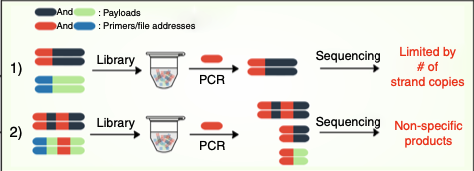
\includegraphics[width=3.5in]{pcrchallenges}
\caption{PCR Challenges}
\label{pcr_challenges}
\end{figure}

\begin{figure}[!t]
\centering
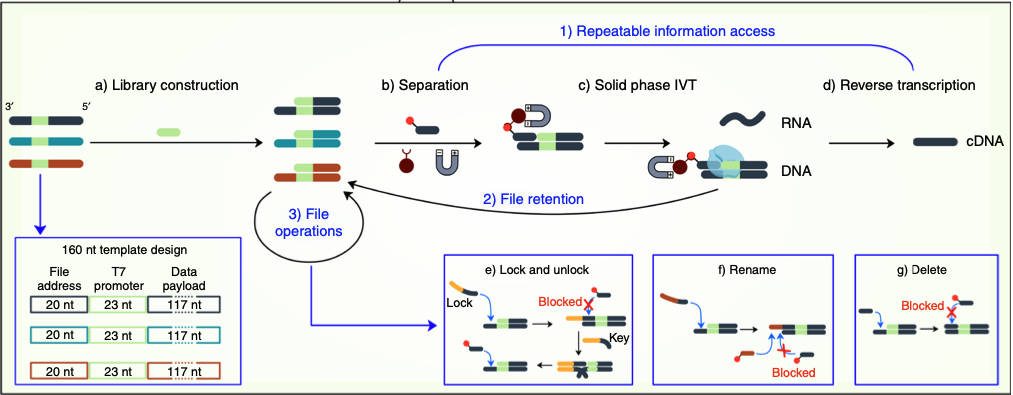
\includegraphics[width=3.5in]{doris}
\caption{DORIS}
\label{doris}
\end{figure}

\section{Comparison}
A purely PCR based approach continues to be the state-of-the-art technique for random access, as it has been reproduced the most often and tested on the largest scales. Although it has been a great start for random access, it by itself is not scalable in regards to database size and physical redundancy \cite{}. 

As argued in the previous section, PCR based random access, although robust, requires physical redundancy because each physical DNA pool can only be accessed once. Chemical handles provide a workaround by enabling the separation of the targeted strand from it's neighbors before sequencing. Nonetheless, this process as presented in \cite{} still relies on PCR for amplification of the data strands. DORIS circumvents this by means of a T7 promoter, meaning that a sequence is copied with an RNA polymerase, leaving the original strand intact and returnable to the original DNA pool, while keeping the other info sequences safe from destructive sequencing.

The original paper using chemical handles was a great leap forward, reducing the need for physical redundancy and providing a promising solution for reusable DNA pools. In particular, unaccessed sequences stay largely intact, apart from the PCR cycles they go through while adding the modified primers to the sample. However, this experiment was done on a small scale and was only able to address 5 distinct files. The same problem faces the T7 promoter based approach, in which the authors did not disclose the amount of data used for testing. While simulations are good for modeling, these novel approaches must both be replicated on larger scales before the approaches can be considered practically scalable as well. 

Nonetheless, all of these methods still rely on PCR as an addressing mechanism, in which it's main goal is to target the correct strand and make it easily readable for the sequencing technology. Future techniques will need to be able to keep existing strands intact, in order to maintain reusability of a DNA storage library. Although this is achievable in theory by chemical handles, it still is a workaround to the current sequencing technology, which gives high error rates and reads all sequences available in a given sample, regardless of what "addresses" one uses. 

An alternative, hypothetical system which has not yet been tested would use DNA microarrays as a random access mechanism. DNA microarrays are essentially grids of DNA binding sites, where each site contains a few (TODO) ss-DNA strands which represent the complements of the address and primer portion of the data we want to retrieve. Combining this with promoters for RNA polymerase would mean one could safely make copies of an entire DNA library, then use microarrays to separate the sequence from it's neighbors. 

\section{Conclusion}
As sequencing costs continue to fall and data growth rates continue to rise, DNA storage will become increasingly more attractive as time goes on. Many steps have been taken to make this a real alternative, but there are still many factors to be improved upon before it can be considered practical (disregarding costs).

It has been shown that basic random access can be achieved using polymerase chain reaction, which continues to be the state of the art method. The encoding methods used are very robust and it can be assured with enough planning and careful encoding that each file is uniquely identifiable and directly accessible. The presented techniques for achieving random access in DNA storage libraries build on top of each other, each bringing forth new research problems to investigate in coming years.

In particular, using chemical handles to physically separate the queried sequences from it's neighbors has been experimentally tested on a small scale and provides significant re-usability of the data pool. It is an open topic as to how this process could be optimized, or if there are any other primer modifications that could allow for even simpler extraction of the matched strands.

It has yet to be tested how the hierarchical primer approach compares to the custom address + RNA polymerase technique. In general, both mechanisms must be replicated on larger scales using real data in order to shift the current paradigm.

Once the RNA polymerase technique proves to successfully combat the problems posed by PCR based random access in practice, new optimization targets can be set. In particular, the viability of RNA polymerase based approaches can be improved upon by further optimizing the re-usability of the system. This would mainly be ameliorated by experimenting with different promoters and different chemical handles as well as the general methods for magnetic extraction and returning of the sequences. 

One thing is clear: for a large one-pot storage of information-bearing DNA strands, a PCR-based approach cannot scale. 




% trigger a \newpage just before the given reference
% number - used to balance the columns on the last page
% adjust value as needed - may need to be readjusted if
% the document is modified later
%\IEEEtriggeratref{8}
% The "triggered" command can be changed if desired:
%\IEEEtriggercmd{\enlargethispage{-5in}}

% references section

% can use a bibliography generated by BibTeX as a .bbl file
% BibTeX documentation can be easily obtained at:
% http://www.ctan.org/tex-archive/biblio/bibtex/contrib/doc/
% The IEEEtran BibTeX style support page is at:
% http://www.michaelshell.org/tex/ieeetran/bibtex/
%\bibliographystyle{IEEEtran}
% argument is your BibTeX string definitions and bibliography database(s)
%\bibliography{IEEEabrv,../bib/paper}
%
% <OR> manually copy in the resultant .bbl file
% set second argument of \begin to the number of references
% (used to reserve space for the reference number labels box)
\begin{thebibliography}{1}

\bibitem{IEEEhowto:kopka}
H.~Kopka and P.~W. Daly, \emph{A Guide to \LaTeX}, 3rd~ed.\hskip 1em plus
  0.5em minus 0.4em\relax Harlow, England: Addison-Wesley, 1999.
  \bibitem{IEEEhowto:kopka}
H.~Kopka and P.~W. Daly, \emph{A Guide to \LaTeX}, 3rd~ed.\hskip 1em plus
  0.5em minus 0.4em\relax Harlow, England: Addison-Wesley, 1999.
  \bibitem{IEEEhowto:kopka}
H.~Kopka and P.~W. Daly, \emph{A Guide to \LaTeX}, 3rd~ed.\hskip 1em plus
  0.5em minus 0.4em\relax Harlow, England: Addison-Wesley, 1999.
  \bibitem{IEEEhowto:kopka}
H.~Kopka and P.~W. Daly, \emph{A Guide to \LaTeX}, 3rd~ed.\hskip 1em plus
  0.5em minus 0.4em\relax Harlow, England: Addison-Wesley, 1999.
  \bibitem{IEEEhowto:kopka}
H.~Kopka and P.~W. Daly, \emph{A Guide to \LaTeX}, 3rd~ed.\hskip 1em plus
  0.5em minus 0.4em\relax Harlow, England: Addison-Wesley, 1999.
  \bibitem{IEEEhowto:kopka}
H.~Kopka and P.~W. Daly, \emph{A Guide to \LaTeX}, 3rd~ed.\hskip 1em plus
  0.5em minus 0.4em\relax Harlow, England: Addison-Wesley, 1999.
  \bibitem{IEEEhowto:kopka}
H.~Kopka and P.~W. Daly, \emph{A Guide to \LaTeX}, 3rd~ed.\hskip 1em plus
  0.5em minus 0.4em\relax Harlow, England: Addison-Wesley, 1999.
  \bibitem{IEEEhowto:kopka}
H.~Kopka and P.~W. Daly, \emph{A Guide to \LaTeX}, 3rd~ed.\hskip 1em plus
  0.5em minus 0.4em\relax Harlow, England: Addison-Wesley, 1999.
  \bibitem{IEEEhowto:kopka}
H.~Kopka and P.~W. Daly, \emph{A Guide to \LaTeX}, 3rd~ed.\hskip 1em plus
  0.5em minus 0.4em\relax Harlow, England: Addison-Wesley, 1999.
  \bibitem{IEEEhowto:kopka}
H.~Kopka and P.~W. Daly, \emph{A Guide to \LaTeX}, 3rd~ed.\hskip 1em plus
  0.5em minus 0.4em\relax Harlow, England: Addison-Wesley, 1999.
  \bibitem{IEEEhowto:kopka}
H.~Kopka and P.~W. Daly, \emph{A Guide to \LaTeX}, 3rd~ed.\hskip 1em plus
  0.5em minus 0.4em\relax Harlow, England: Addison-Wesley, 1999.
  \bibitem{IEEEhowto:kopka}
H.~Kopka and P.~W. Daly, \emph{A Guide to \LaTeX}, 3rd~ed.\hskip 1em plus
  0.5em minus 0.4em\relax Harlow, England: Addison-Wesley, 1999.
  \bibitem{IEEEhowto:kopka}
H.~Kopka and P.~W. Daly, \emph{A Guide to \LaTeX}, 3rd~ed.\hskip 1em plus
  0.5em minus 0.4em\relax Harlow, England: Addison-Wesley, 1999.
  \bibitem{IEEEhowto:kopka}
H.~Kopka and P.~W. Daly, \emph{A Guide to \LaTeX}, 3rd~ed.\hskip 1em plus
  0.5em minus 0.4em\relax Harlow, England: Addison-Wesley, 1999.
  \bibitem{IEEEhowto:kopka}
H.~Kopka and P.~W. Daly, \emph{A Guide to \LaTeX}, 3rd~ed.\hskip 1em plus
  0.5em minus 0.4em\relax Harlow, England: Addison-Wesley, 1999.

\end{thebibliography}




% that's all folks
\end{document}


